\chapter{Introduction} \label{ch:intro}

\blindtext

\section{Tikz}

In \cref{fig:dataflow} is an example of a tikz drawing. Use the \textbackslash cref or \textbackslash Cref command to reference anything that \textbackslash ref would otherwise be used for. \textbackslash Cref is for capitalized references and \textbackslash cref is for lower case refrences.  This document forces the capitalization of figures, tables, listings, sections, and chapters.  This can be changed in the preamble with the \textit{cleveref} package. Tikz is a useful tool for drawing diagrams, and I highly suggest learning it.

\tikzstyle{basic} = [rectangle, rounded corners, minimum width=2cm, minimum height=1cm,text centered, draw=black]
\tikzstyle{arrow} = [thick,->,>=stealth]
\begin{figure}[ht]
\centering
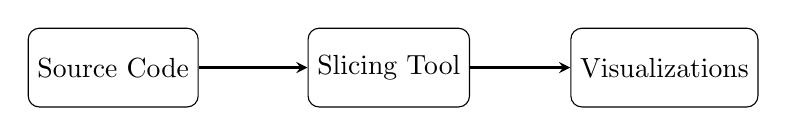
\begin{tikzpicture}[node distance=3.5cm]
\node (src) [basic] {Source Code};
\node (slice) [basic, right of=src] {Slicing Tool};
\node (viz) [basic, right of=slice] {Visualizations};

\draw [arrow] (src)--(slice);
\draw [arrow] (slice)--(viz);

\end{tikzpicture}
\caption{The flow of data in \textbf{vizSlice}}
\label{fig:dataflow}
\end{figure}




\section{Figures}

In \cref{listing:srcMLInput} is an example of a code listing.

\begin{listing}
		\vspace{\baselineskip}
			{\small
			\inputminted{cpp}{supportingDocs/radius-func-cpp.tex}
			}
            \caption{Example input to srcML}
            \label{listing:srcMLInput}
  		\vspace{\baselineskip}
\end{listing}

In \cref{fig:brushedPara} is an example of an image figure. 

\begin{figure}[ht]
    \centering
    \includegraphics[width=\textwidth]{brushedPara.PNG}
    \caption{An parallel coordinates visualization using    brushing\cite{paracoord}}
    \label{fig:brushedPara}
\end{figure}

\blindtext